%!TEX program = xelatex
% 完整编译: xelatex -> biber/bibtex -> xelatex -> xelatex
\documentclass[lang=cn,a4paper]{elegantpaper}

\title{作论文模板}
\author{Zhengqing ZHOU \thanks{北京大学} \\ Peking University \and Zhengqing ZHOU \\ PA Technology}
\institute{\href{https://pe.pku.edu.cn/}{体育教研部}}

\version{0.10}
\date{\zhtoday}

\usepackage{setspace}
\usepackage{amsmath}
\usepackage{amssymb}
\usepackage{graphicx}
\usepackage[utf8]{inputenc}
\setlength{\parskip}{0.125in}%段间距
\usepackage[autostyle]{csquotes}

% Packages for automated tables
\usepackage{tabularx}
\usepackage{standalone}
\usepackage{pdflscape}
\usepackage{iftex, fancyhdr, hyperref, enumitem, fancyvrb, hologo, multirow, booktabs, bigstrut, tabularx, tocloft}
\usepackage{lipsum}

\usepackage{changes} %批注
\usepackage{bm}
\hypersetup{colorlinks = true, allcolors = blue}
\pagestyle{fancy}\fancyhf{}\cfoot{\thepage}
\renewcommand*{\headrulewidth}{0pt}
\ctexset{linestretch = {\maxdimen}}
\setlength{\hfuzz}{3pt}
\setlist{nolistsep}

% 本文档命令
\usepackage{array}
\newcommand{\ccr}[1]{\makecell{{\color{#1}\rule{1cm}{1cm}}}}
\addbibresource[location=local]{reference.bib} % 参考文献,不要删除

\begin{document}

% Title Page
\begin{titlepage}
\clearpage\maketitle
\thispagestyle{empty}

\begin{abstract}
本文为的说明文档。此模板基于 \LaTeX{} 的 article 类,专为工作论文写作而设计。设计这个模板的初衷是让作者不用关心工作论文的格式,专心写作,从而有更加舒心的写作体验。如果你有其他问题、建议或者报告 bug,可以在 \href{https://github.com/ElegantLaTeX/ElegantPaper/issues}{GitHub::ElegantPaper/issues} 留言。如果你想了解更多 Elegant\LaTeX{} 项目组设计的模板,请访问 \href{https://github.com/ElegantLaTeX/}{GitHub::ElegantLaTeX}。
\keywords{Elegant\LaTeX{},工作论文,模板}
\end{abstract}

\end{titlepage}
    \thispagestyle{empty}
	\newpage
    \phantomsection\addcontentsline{toc}{section}{摘要}\tolerance=500 %将摘要放进目录
    \tableofcontents
    \setcounter{page}{1}
	\newpage

% 理论、变量、处理手法、基本结论
	\section{基本材料} \label{sec:text}
	\subsection{重要的概念与新变量}

儿童时期的家庭环境和培育水平决定了个人一生的技能基础,是人类发展的 关键因素(Heckman and Mosso,2014)。在解释经济地位的代际流动中起着关键作用,在有利和不利环境中成长的儿童, 其人力资本的差距早在入学之前就已经出现;而 传统的教育政策无法完全弥补弱势家庭中父母投资不足造成的伤害。不同家庭背景成长起来的儿童,面临着所谓 的“命运岔路”,也即人力资本投资中的机会不平等。

【me】人力资本是个人发展的重要决定因素,技能和能力(Skills and abilities)是重要的组成维度。传统的人力资本研究框架中\footnote{以 Theodore Schultz、Gary Becker、Jacob Mincer 等经济学家为代表建立的人力资本理论是围绕人力资本的投资和收益而建立起来的。 该理论的核心是,劳动者可以通过教育、培训、保健等方式提高其生产能力,进而提高未来的收入。最初,人力资本理论的研究主要集中在传统上被认为与教育 和收入等结果相关的认知技能上。20 世纪末期,随着心理学家对能力内涵研究的进一步深入,人力资本理论逐渐从“以认知能力为核心”拓展为包括“认知与 非认知能力”。Bowles et al. (2001)重新阐释了这一概念,强调了非认知能力的 经济价值。最近的研究都显示了非认知能力,如毅力、耐心、社交能力以及其他人格和行为特征,是儿童期和成年期结果的重要决定因素(Heckman and Rubinstein,2001;Heckman et al.,2006,2011;Heckman and 2 Mosso,2014)。 而有关美国社会流动性的研究表明,不同家庭背景成长起来的孩子面临着所谓的“命运岔路”(Chetty et al.,2014a,2014b,2018a,2018b)。},经济学家聚焦在个体教育水平差异是否可以解释市场中劳动生产率和劳动报酬的差异。研究人力资本的意义。经济学家认为,人力资本提高会提升劳动生产率。




【me】实证操作中,由于能力无法直接观察,一般将教育程度作其代理变量,其隐含的假设是教育水平差异可以准确反映个体能力差异。然而,这等价于片面地把能力等同于认知能力,而忽视了非认知能力(责任心、自尊)的经济价值,限制了人力资本理论的解释力。

【me】家庭培育和教师培育一直是公认的人力资本形成重要因素,但其形成机制缺处于“黑箱”状态。正如《科尔曼报告》(1966)所强调,解释学生成绩的绝大部分差异是家庭特征而非学校特征。

全生命周期的生活运动。现代父母大部分是重视青少年体力活动发育,

孩子在校园不运动是父母培育的意识不够,还是环境使然?没有证据。
    接受课外班的孩子的体力活动 vs 不接受课外班的孩子的体力活动

对于经济学家所描述的非认知能力这一概念,心理学家更偏好用人格心理学中的人格(Personality)或人格特质(Personality trait)的概念来替代。一个被广泛接受的人格特征分类 是五因素模型(Five-Factor,简称 FF)。根据 2005 年 Nyhus 和 Pons 的定义,该 模型包括以下因素:宜人性、责任心、情绪稳定性(也称神经质)、外倾性和自主性。

【me】非认知能力与认知能力的区别?sport对它的影响?与对认知能力的区别。
许多研究记录了非认知技能在解释学业成就、劳动力市场成功和其他重要生活成果方面的重要性。(Heckman 和 Rubinstein 2001 年;Flossmann、Piatek 和 Wichert 2008 年;Bertrand 和 Pan 2013 年; Heckman、Pinto 和 Savelyev,2013 年;Segal,2013 年)。为了解学校影响在非认知结果中所起的作用,我们将重点放在中学时期,因为人们认为这是非认知技能发展和成熟的年龄(Borghans 等人,2008 年;Heckman 和 Kautz,2013 年)。

【new】也就是说,学生类型(运动型+学A)、(运动型+学B)。。。
还是学生体型【肥胖型+学A】还是【偏瘦型+运动能力】

现实问题是运动能力如何衡量?CEPS是否支持?

教师是否偏爱,一位爱运动、同性别更多的支持,在学业上有更好的表现?

教师是否偏爱同性学生,以便他们对男女学生给予不同的关注或反应?或者,在相同的教学行为下,女孩和男孩对指令的反应和回应方式是否不同?在设计减轻学校性别差异的政策时,了解这些机制很重要。
现实情况是,学校教师的性别构成很难改变。教师行为和学生信念的独特数据来直接测试教师行为如何因学生性别而异,以及学生与学习相关的信念和动机如何受到教师性别的影响,从而深入了解这个问题。



【new】接受早期投资的儿童会比那些失去早教机会的儿童积累更多的人力资本存量。对班级内的能力同伴效应(Ability Peer Effects)(也即早期投资的溢出效应)进行实证检验。

家庭的培育(Parenting)的理论框架是什么?AER那篇。

\subsection{重要理论}

生命周期的早期影响。儿童早期干预的证据主要来自美国等发达国家的干预项目。但是,由于这些 干预措施在处理方式,环境和持续时间方面各不相同,因此很难直接比较以确定 其相对有效性。

家庭投资与儿童发展。大量经验证明,家庭收入与子女成绩密切关系。在儿童 发展过程中,发现(母亲和父亲的)时间投入比货币支出更重要。等儿童成长到青春期,财务约束才显得更为重要(并且向家庭转移资金更为有效)。家庭财富只是家庭环境的其中维度。其他方面,如父母教育程度,养育能力,利他主义,和居住环境等。

留守儿童与流动家长面临强烈的时间约束。

庭养育方式与儿童发展。

同伴效应对人力资本形成的溢出效应。理论基础是社会互动(Socila interaction )

以上理论,并不意味着孩子进入青少年阶段后,父母的影响就不重要了。

与周正卿(2022)不同的peer effect 效应:首先, 定义同伴效应 
$\bar{\theta}_{-i, t})$ 捕捉了第 $i$ 个孩子所对应的平均同伴技能:
$$
\bar{\theta}_{-i, t}=\frac{1}{\sum_{j \in N_e} L_{i, j, t}} \sum_{j \in N_e} L_{i, j, t} \cdot \theta_{i, t}
$$
其中 $L_{i, j, t}$ 是一个指示函数, 如果孩子 $\mathrm{i}$ 和孩子 $\mathrm{j}$ 是朋友, 那么 $L_{i, j, t}$ 赋值为 1 ; 反之则为0。

模仿等式 (3.13), 对人力资本形成的同伴效应进行如下建模:
$$
\mathrm{d}_{i, t+1}=\left[\delta\left(I_{i, t}\right)^\pi+(1-\delta)\left(\bar{\theta}_{-i, t}\right)^\pi\right]^{\frac{1}{\pi}}
$$
其中, 家庭投资与同龄人之间互补性/替代性由 $\pi$ 定义。当 $\pi=1, I_{i, t}$ 和 $\bar{\theta}_{-i, t}$ 是完
全替代。当 $\pi=-\infty, I_{i, t}$ 和 $\bar{\theta}_{-i, t}$ 是完全互补。对儿童 $\mathrm{i}$ 而言, 第 $\mathrm{t}$ 期的父母的人力资本 投资 $I_t$ 与同伴们的平均技能之间的动态互补性来自人力资本的自我生产性。如果 同伴的人力资本水平可以与学生的家庭投资形成互补,那么就意味着处于优势境 遇的父母可以通过选择孩子的伙伴,例如购买学区房、择校等投资行为,通过增 加的隔离来强化这一互补机制的效果,也即实现“近朱者赤”。

\subsection{数据处理}

并将样本限制在那些遵循随机分配规则的学校,本研究估计了早期人力资本投资的直接效应和溢出效应。具体而言,本研究将家庭早期投资差异定义为是否接受学前教育,也即在儿童成长的第一阶段(学龄前)是否让子女接受学前教育(幼儿园),从而考察学生接受学前教育与否,以及班级内接受学前教育的学生的比例如何影响学生第二个阶段(中学期间)的认知技能和非认知技能发展。


CEPS确保如何是随机分班。本研究主要采用了CEPS2013-2014年的基线调查数据。学校数据往往存在自选择的问题,也即由于潜在可观测或者不可观测的因素,导致学生被分配到特定的班级,这就会导致在估计教育生产函数时存在偏误。本研究的理想状态是,学生的个人特征和班级的特征不会影响学生的分班结果,也即学生们是被随机分配到不同班级的。虽然《中华人民共和国义务教育法》中严格要求初中学校不得在学校中分设重点班和非重点班,但有些学校在实践中可能没有严格遵守这一规定。

为此,本研究采用如下步骤来筛选出可能没有严格遵守随机分配规则的学校。首先,每位校长都会被要求回答如下两个问题,一是7年级学生入学时是否随机或平均地分配到班级中去,二是这些学生在随后的中学期间(也即8年级和9年级)是否会被再次分班。本研究排除了那些报告在7年级非随机分配学生,或者在8年级和9年级时重新分配学生的学校。第二,班主任会被要求报告学生是否被按考试成绩进行分配。本研究也放弃了那些班主任报告的按成绩分班的学校。最后,本研究的样本包含了来自64所学校256个班级的约1万多名7年级和9年级的学生。

Gong 2018是如何随机分班的?
【好处】这使我们能够减轻潜在的选择问题——例如,成绩优异或积极性更高的女学生更有可能被分配给女教师。通过比较女教师和男教师教授的女孩和男孩的结果,我们能够估计教师性别是否以及如何以不同方式影响男女学生的结果。

【Gong】使用聚合的方法对8个认知变量,主成分分析。然后分为精神压力水平和社会适应
除了估计教师性别对这八个非认知变量的影响外,我们还遵循Kling、Liebman和Katz(2007)提出的汇总方法来了解教师性别的总体影响。具体来说,我们首先使用主成分分析方法,将八个非认知变量分为两类,即精神压力水平和社会适应与满意度水平(详情见附录A;附录A,B可在线查阅)。然后我们计算每个类别的平均效应大小(AES),它是其组成部分的Z-cores的加权平均值。当结果也有特异性变化时,这种汇总提高了检测特定结果中一致的效果的统计能力。

Specifically, we define the AES of teacher gender on noncognitive category $c$ as $\mathrm{AES}_c=\left(1 / n_c\right) \sum_{n=1}^{n_c} e_{k c} / \sigma_{k c}$, where $n_c$ is the number of outcomes in category $c$ (e.g., four for the category of mental stress), $e_{k c}$ is the estimated effect for outcome $k$ of category $c$, and $\sigma_{k c}$ is the standard deviation of the outcome variables.



→→ 幼儿时期父母体育培育意识对青少年社会适应的影响?

【【重头戏!!!】】随机分配的方式!
我们的研究问题涉及教师性别对学生成绩的影响。因此,了解学生与教师和课堂的匹配方式对于我们的评估和分析至关重要。中国的中学使用各种方法分配学生。在一些学校,学生在开始第一学年之前参加分班考试,他们的分数用于将他们分配到教室。在其他学校,学生是根据当地居民身份分配的。最近,越来越多的学校开始采用随机分配的方式将学生分配到教室。教育部大力提倡这种方法,以确保所有学生在义务教育期间(直至九年级)享有平等和公平的机会。使用随机分配的学校通常依赖于一个计算机程序,该程序可以包含有关班级规模、性别\footnote{Our observed female dominance in secondary school teachers is a global phenomenon. See, e.g., Holmlund and Sund (2008) and Winters et al. (2013).s}、移民身份和其他方面,以确保随机化过程中的适当平衡。或者,如果入学人数较少且易于管理,则邀请新生的家长抽签决定孩子的班级安排。在这些情况下,一旦确定了学生抽签,校长和学科教师也会抽签决定他们将教授和管理哪些教室。
使用我们的标准,我们发现 2014 年 CEPS 数据库中 59.8\% 的学校随机分配教室,转化为 67 所学校 208 间教室的 8,988 名学生的样本。由于我们样本中的每个学生都被随机匹配到班主任和学科教师,并在接下来的 3 年里留在同一个教室,因此我们的样本减轻了有关学生自行选择班级或教师的任何潜在担忧。

标准是基于教师问卷调查中的报告。对于第一个条件,所有学校的校长都被要求报告他们使用以下哪种分配规则来安置学生。(a) 入学前的考试成绩,(b) 学生的居住状况,(c) 随机分配,或(d) 其他因素。其次,这些校长被问及他们的学校是否为8年级和9年级重新安排教室;我们排除了那些这样做的学校。最后,每个校长都被问及所教年级的学生是否按考试成绩分配;同样,如果有校长回答是,我们就放弃整个年级。

人们可能会担心家长会像 STAR 实验那样抱怨教室随机化的结果,并要求他们的孩子搬到其他教室。我们在调查数据中没有直接信息。然而,学校校长被问及家长是否要求将他们的孩子分配到特定教师的班级,评分标准为 1(完全不相关)、2(不相关)、3(稍微相关)或 4(绝对相关)。在通过随机化限制的 67 所学校中,只有一所学校的校长报告了 4(绝对相关),另外九所报告了 3(轻微相关)。排除这 10 所可能重新分配学生的学校并不会改变我们的估计结果。



流动人口、回流人口

复合变量:家庭社会地位,综合评分,连续型
→ 家庭支持

----------------------------------------------------------------


 在流动人口中,SES 对 跨群体朋友数量 为 +

 在本地人口中,SES 对 跨群体朋友数量 为 -

 在全人口中,SES 对 跨群体朋友数量 为正 0 


运动能力


跨群体(某一类)朋友数量
% Introduction引言
	\section{引言} \label{sec:introduction}
	定期参加体育活动(PA)对于维持整个生命周期的健康和福祉至关重要。大量证据显示在儿童和青少年中,身体活动可以显著改善身体健康(心肺和肌肉健康)、骨骼健康、认知结果(学业成绩和执行功能)、心理健康(抑郁症状机减少)以及肥胖症状减轻(WHO,2020),但在发展中国家,许多儿童仍旧无法得到充足的锻炼。当前,中国青少年的心理健康问题不容忽视。据估算,约7%~30%的中学生存在焦虑、抑郁等心理健康问题。数据显示......这一现象也引起中国政府高度重视,《“健康中国2030”规划纲要》提出要实施青少年体育活动促进计划,培养青少年体育爱好。

青少年缺少PA的一个重要的原因是其复杂、多样的决定因素,包括个人、家庭、学校和社会等多种环境因素会影响儿童和青少年行为(Biddle和Asare,2011年;Mitchell等人,2016年)。近30年的改革开放,中国一方面经历了快速的城市化和工业化发展,另一方面见证了时间最大规模的流动人口。城乡间大规模的人口流动为中国城市发展带来充足的人力和智力支持,同时也使得流动人口与本地居民的社会融入问题日益突出。事实上,这种社会空间的隔离也进一步导致流动儿童面临较为严重的城市融入问题。并且在心理发展、教育期望、学业表现等方面与本地儿童相比均处于明显的劣势(周皓、巫锡炜,2008;柳建坤等,2020;谢建社等,2011)。因此,分析和考察流动儿童和本地儿童的社会融合对青少年的健康发展、促进教育公平和城市社会的可持续发展具有重要的现实意义。为了改善家庭经济状况和生活质量,大量农村劳动力选择进程务工,同时子女也随父母远离家乡,成为了流动儿童。

作为青少年行为中啊哟关于流动儿童其父母影响运动参与问题,目前的研究或者直接分析影响流动儿童社会融入的现实障碍和影响因素。不可否认,这些研究对于我们理解流动儿童的社会融入问题具有重要意义,但它们大多忽视了流动儿童社会融入过程中的另一个重要问题——社会交往,更确切地说,是流动儿童与本地儿童之间的友谊问题。学校和家庭是青少年日常生活中最为重要的两个生活场域。学校不仅为青少年提供了适应未来工作和生活所必备的知识和技能,也同时为他们建立同伴关系和发展友谊提供了一个相对制度化的社会交往空间。然而,不同学校,甚至学校中不同班级之间,在群体构成、同辈互动情境等方面往往存在显著差异。因此,青少年在不同的学校和班级所面临的社会交往环境可能会完全不同,进而发展出迥异的社会交往关系(McFarland,etal.,2014)。更进一步说,这种社会交往关系还可能会因为青少年社会身份(如流动儿童和本地儿童)的差别而存在较为明显的差异。同样,作为社会化的另一个重要场所,家庭也对青少年的社会交往有重要影响。不同阶层的父母所持有的价值观念以及亲子间互动的方式都会潜移默化地影响青少年社会交往的方式和偏好(VanTubergenandSmith,2018)。,却只有少量国内学者注意到这一问题(史晓浩、王毅杰,2010;王毅杰、史晓浩,2010),而且也没有进行严谨的实证检验。

基于此,本文旨在考察同伴效应对青少年体育锻炼是否构成因果关系。基于国内范围最广的教育追踪调查数据,笔者使用工具变量方法消除了潜在的同伴效应内生性问题,发现同伴效应对初中生的体育锻炼时间具有正向显著影响。同时验证了了王富百慧等(2018)以及权小娟和卢春天(2020)的假设,即同伴支持同样会对个体锻炼时间有显著正向促进作用。进一步机制分析发现,班级运动氛围在同伴效应影响青少年体育锻炼时间路径中起中介作用,一方面同伴效应会显著正向促进班级运动氛围提升,另一方面,班级运动氛围同样提高个人运动参与。

综上所述,本文边际贡献主要体现在两个方面:首先,在理论上将青少年个体运动行为与教育学中经典的同伴效应问题进行连接,呼应Manski(1993,2000)等学者指出的内生性问题对同伴效应估计中造成的偏误影响,揭示了本领域研究“重相关,轻因果”传统而常忽略的遗漏变量问题。其次,实证方面,建立在教育追踪调查的数据优势允许我们使用基期调查时的同伴数据作为同伴效应的替代测量,同时将基期同伴父母的运动陪伴作为当期同伴效应的工具变量,获得了同伴效应的纯净估计值。最后,对同伴效应影响青少年体育锻炼行为的机制深入分析,班级运动氛围中介效应能够解释近20\%的总效应影响,该结论不仅从再次从学理层面验证了同伴效应对青少年体力活动促进的重要性,而且为从实践层面为合理引导学生参与体育锻炼提供了政策启示。

余下的部分安排如下,本文的第二节是文献回顾,第三节是研究设计,第四节是数据来源与数据描述,第五节是研究结果与分析,最后给出本文的结论和政策建议



基于上述讨论,本研究将着重检验当前中国初中教育阶段家庭背景和学校的班级情境对流动儿童和本地儿童之间跨群体交往的影响差异。具体来讲,通过分析“中国教育追踪调查”(CEPS)数据,本文试图回答以下问题:第一,家庭社会经济地位对青少年的跨群体交往的影响和群体差异;第二,班级情境,尤其是班级中的群体构成、同辈群体、外部群体对青少年的跨群体社会交往起到何种作用,以及对流动儿童和本地儿童又有何种差异虽然这些流动儿童会与父母生活一起,但让他们受父母工作、家庭环境等因素变化,对校园活动那个产生影响。家庭、学校和社会是儿童青少年进行体育运动的三个主要场域,其中家庭是个人社会化最初的场所,家庭教育是学校教育和社会教育的基础,大量研究已经证明,在早期的体育兴趣培养中,家庭相对于学校和社会的影响是最大的。家长的期望信念、价值信念与子女的教育期望会与PA呈高度正相关。家长对子女要求越高,与教师越匹配就荣促进参加PA。家长与子女的互动越多,对PA有正向作用。行为,家长行为会诱导孩子模仿。家长的社会资本越多,孩子可能会承接家长的交流能力,从而促进PA。同伴的家长特征,就会促进PA。比如同学的家长,陪同孩子参加课外体育锻炼、家长经常与孩子一起娱乐,都会促进孩子参加体育锻炼。中介方面,认可度较高的家长教养方式、家庭社会资本、家长教育程度、家庭经济条件也是显著因素。家庭体育是青少年行为养成的重要依托。父母作为家庭主要成员,对青少年体育锻炼参与度有广泛的影响。然而,青少年在行为养成时期,家庭因素影响占比逐渐增大。因此这一时期要格外注重家庭体育环境的建设和优化。

% Section文献综述
	\section{文献回顾} \label{sec:review}
	\input{./sub/review.tex}
% Section文献综述
	\section{研究设计} \label{sec:design}
	\input{./sub/design.tex}
% Section方法
    \section{数据来源与数据描述}\label{sec:data}
	\input{./sub/sample.tex}
% Section实证结果
    \section{研究结果与分析}\label{sec:results}
	\subsection{基准回归}
%
%\begin{center}
%\begin{figure}[h]
%\centering
%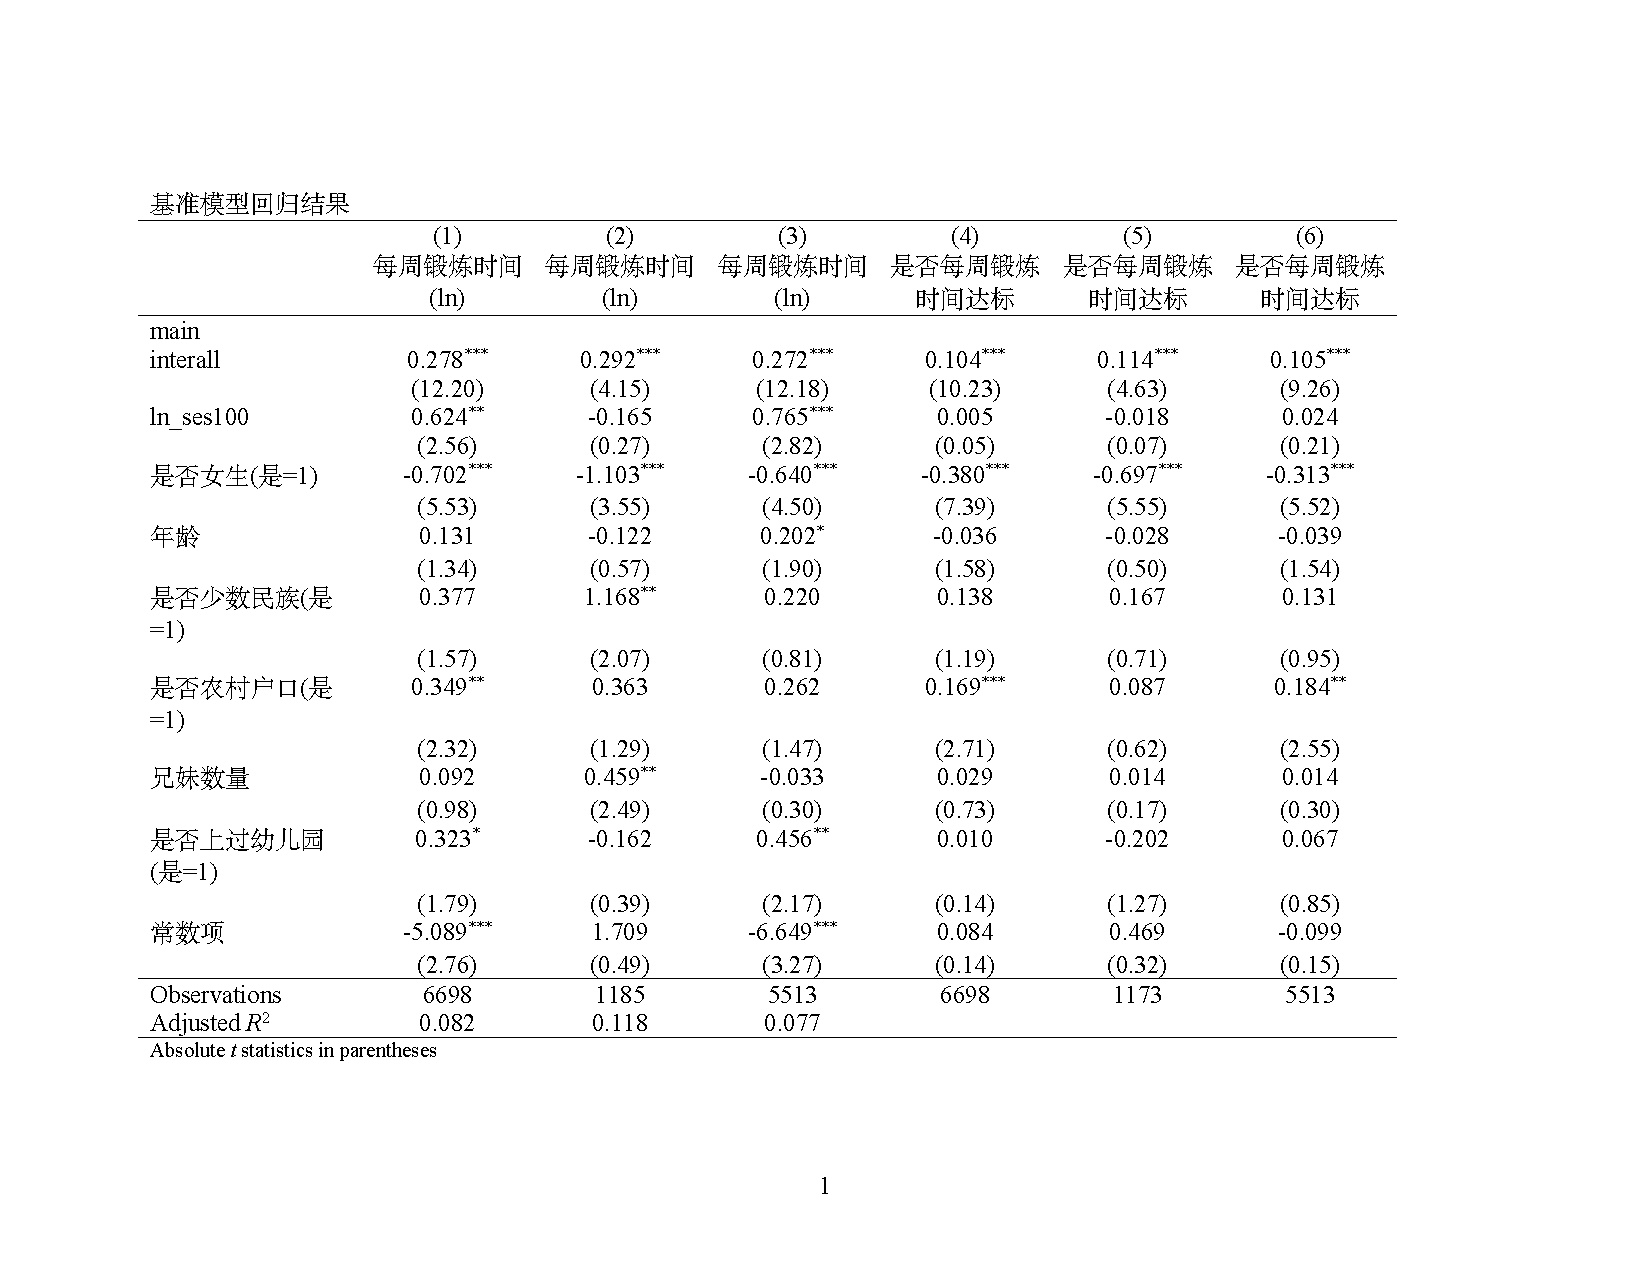
\includegraphics[width=1.25\textwidth]{figures/basigreg01.pdf}
%\caption{基准回归模型}
%\label{fig:}
%\end{figure}
%\end{center}

\subsection{异质性分析}
% Conclusion
	\section{结论} \label{sec:conclusion}
	\input{./sub/conclusion.tex}
% References
	\newpage
%	\bibliographystyle{apa}
%	\bibliography{}
	\nocite{*}
	\printbibliography[heading=bibintoc, title=\ebibname]
% Appendix
	\newpage
	\appendix
	\section{附录} \label{sec:appendix}
	
% FIGURES
\subsection{Figures}

\begin{figure}[H]
\caption{}
\centering
%\includegraphics[scale=1]{../../output/}
\label{fig:}
\end{figure}


% TABLES
\newpage
\subsection{Tables}

\begin{table}[H]
\caption{}
\centering
\begin{threeparttable}
%\input{../../output/}
\end{threeparttable}
\label{tab:}
\end{table}

	\addappheadtotoc

\end{document}